%%%%%%%%%%%%%%%%%%%%%%%%%%%%%%%%%%%%%%%%%%%%%%%%%%%%%%%%%%%%%%%%%%%%%%%%%%%%%%%%%
%
%  Bachelorarbeit Adler Tilman 01.06.2015
%  "Titel"
%  Lehrstuhl fuer Mustererkennung, FAU Erlangen-Nuernberg
%
%%%%%%%%%%%%%%%%%%%%%%%%%%%%%%%%%%%%%%%%%%%%%%%%%%%%%%%%%%%%%%%%%%%%%%%%%%%%%%%%%

% ++ LME LateX Dokument
%    Die Verwendung der option "german" bindet german.sty ein.
%    For english papers, use the "english" option and talk to your advisor.
\documentclass[english,bt]{package/lmedoc}
%\documentclass[english,bt]{lmedoc}

\usepackage{hyperref}

% ++ Umlaut Unterstuetzung
%    Paket "inputenc" kann verwendet werden, um z.B. Umlaute oder das scharfe S
%    direkt (als Nicht-ASCII-Zeichen) einzubinden. Dabei auf die korrekte
%    Kodiermethode achten (z.B. Linux: latin1)!
\usepackage{fontspec}
\usepackage{CJKutf8}
\setmainfont[   Path = fonts/,
                BoldFont = BookmanOldStyleBold.ttf,
                BoldItalicFont = BookmanOldStyleBoldItalic.ttf,
                ItalicFont = BookmanOldStyleItalic.ttf]{BookmanOldStyle.ttf}


% ++ es werden keine underfull hboxes als Fehler ausgegeben,
%    da das ja nur heißt, dass die Seite noch nicht ganz voll ist
\hbadness=10000


\pagenumbering{roman}

\bibliographystyle{package/galpha1a}
\begin{document}
\clearpage
  \begin{deckblatt}
    \Titel{Titel}
    \Name{Adler}
    \Vorname{Tilman}
    \Geburtsort{N"urnberg}
    \Geburtsdatum{16.12.1989}
    \Betreuer{Vincent Christlein}
    \Start{01.01.2015}
    \Ende{01.06.2015}
  \end{deckblatt}


\cleardoublepage

Ich versichere, dass ich die Arbeit ohne fremde Hilfe und ohne Benutzung
anderer als der angegebenen Quellen angefertigt habe und dass die Arbeit
in gleicher oder "ahnlicher Form noch keiner anderen Pr"ufungsbeh"orde
vorgelegen hat und von dieser als Teil einer Pr"ufungsleistung
angenommen wurde. Alle Ausf"uhrungen, die w"ortlich oder sinngem"a"s
"ubernommen wurden, sind als solche gekennzeichnet.
\\

Die Richtlinien des Lehrstuhls f"ur Studien- und Diplomarbeiten
habe ich gelesen und anerkannt, insbesondere die Regelung des
Nutzungsrechts. \\[15mm]
Erlangen, den \today \hspace{6.0cm} \\[10mm]

\cleardoublepage

\begin{center}
\bfseries
"Ubersicht
\normalfont
\end{center}


\vspace{5.0cm}

\begin{center}
\bfseries
Abstract
\normalfont
\end{center}

\cleardoublepage

\tableofcontents

\cleardoublepage \pagenumbering{arabic}

%!TEX root = ../Thesis.tex

\chapter{Introduction}
	\section{Motivation}
	\label{introduction-motivation}
	The game of Go (Japanese \begingroup\setmainfont{Droid Sans Japanese}\small\begin{CJK}{UTF8}{min}囲碁\end{CJK}\endgroup ) is ancient. It is actually older than Christianity and chess. However even though its rules are simpler than the rules of chess it is -- outside of Asia -- not nearly as wide-spread as the latter. When learning Go one comes to a certain point where one single error often decides the whole game. Often the winning player will be able to remove many of his or her opponent's pieces from the board resulting in a devastating defeat. This can be quite frustrating and it is hard to learn from such mistakes because they often manifest not until some moves after they have been made.

	The solution to this is obvious: Record a game and analyze it later, maybe resume it at the questionable move and see if it would have turned out otherwise. While there are advanced players who can ''store'' an entire game in their memory most have to rely on a notation on paper, pocket computers or mobile apps, especially new players. As this process drains on concentration many players tend to not note games.

	There are ways to store board games in an automated fashion, not requiring any interaction by the players. For chess there are specialized boards (DGT chess boards) starting at around 20€, which usually have special (magnetic) pieces\cite{bulsink2001device} or small holes with light sensors. They automatically record a game and send the data to a computer, mobile device or other hardware for display and analysis. However for Go there is -- to our knowledge -- no such thing. Also, the need for specialized hardware makes a solution like this very unappealing.

	What makes the situation worse is that while there is a notation called Kifu (Japanese \begingroup\setmainfont{Droid Sans Japanese}\small\begin{CJK}{UTF8}{min}棋譜\end{CJK}\endgroup ) for the recording of games it is -- again outside of Asia -- not very widespread and no numerical system as in chess (where the columns and rows are determined by a number and a letter) has been generally accepted. Ideally a recording system would save the moves in an independent fashion that makes it easy to transfer into the existing systems' formats or choose one system and save it in its data format. Once such a system exists there are other applications that can be thought of, like playing against a computer or via the internet another human and using real pieces in the process. Anyhow it might lead to more players successfully learning how to play Go (well) and thus contribute to its spread in the western world, if just a little. %TODO: Uebergang

	The ubiquity of mobile devices with built in cameras lets one solution appear very attractive: Have a mobile application record the game, analyze it via a computer vision application and save the result when it detects a new move. This	work intends to provide such a solution and show the efforts taken to create it.

	After presenting related work and possibly related patents we will first describe the part of the application that does the actual detection and go on to the integration of it in an Android app. Thereafter we will discuss impact of different algorithms that have been evaluated regarding detection quality and speed and provide an assessment to what extent the goal of an automated recording device for Go games has been reached. We will conclude with an outlook on possibilities for future work improving upon the solution at hand and a summary of this work.


	\section{Related Work}
	\label{introduction-work}
	The detection and augmenting of board games in general is illustrated by Eray Molla and Vincent Lepetit \cite{molla2010augmented}, who demonstrate the successful tracking of colored pawns on a Monopoly™ board.

	More closely related is  Steven Scher's, Ryan Crabb's and Jamie Davis's work \cite{scher2008making} who collect samples of a Go-board using a fixed camera in regular intervals. They detect the grid in the first image using Hough transformation to generate the board's grid. Afterwards they classify intersections (as ''black'', ''white'' or ''empty'') by template images and use a Markov model to remove errors in the single images by modeling the detected state of every image according to the game rules.

	This approach yields high accuracy when capturing whole games and performing the detection asynchronously. On a mobile device this is not ideal as it drains the battery at a time the user does not expect it to. Also movement of the camera or the board is not supported at all as detection of the grid is only performed on the first image. However smart phones as a multi purpose device should be relocatable at least within a certain range, for example to take a call and then replacing the phone.
	\\

	Similarly Teemu Hirsim"aki \cite{hirsimaki2005extracting} uses the Hough space to find parallel lines near the center of the image. He will then use this information in conjunction with the original image filtered for edges to build the board grid by solving a minimization problem on them. Intersections are classified by relating the median brightness to the median value in a certain window.

	While the author assumes the approach can be used on consecutive frames one problem when using only line detection remains: during later phases of the game many stones will be placed especially in the center of the image. The lines are occluded and there's no way left to detect the board.
	\\

	Alexander K. Seewald \cite{seewald2010automatic} managed to circumvent this by detecting the intersections using the SIFT algorithm specifically during endgame situations. These are then classified (as before but additionally as ''empty inside the grid ┼'', ''empty on the edge ┬'' and ''empty on the corners ┐'') by an SVD and further refined by estimating the board position using the corners and classifying the previously missed stones by average brightness.

	While he solved the problem of detecting end game states this came at the price of performance. With five seconds runtime on a PC for an 8 by 8 grid this solution seems unpractical for slower mobile processors.

	\section{Related Patents}
	\label{introduction-patents}

	... === TODO === ...


\cleardoublepage
%!TEX root = ../Thesis.tex

\chapter{Detecting the board}
	\label{detector}
	When looking at a Go board what first catches one's eye are the lines. As we said before, though, relying solely on lines for the detection of the grid will probably fail in endgame situations. Therefore our algorithm uses them only to find intersections and tries to fill in gaps by adding information about pieces, too. This was born out of the idea that what is actually interesting are not the lines, but their intersections and a piece will always lie reasonably close to one. We also rely on the user placing the camera or the board such that the center of the board is located in the center of the screen.

	Our implementation was based on the OpenCV framework in its current version 2.4.10 and where not noted otherwise all detection has been performed on x86\_64 architecture. As described in chapter 3 this does not seem to provide different results than execution on mobile devices (i.e. ARM architecture), for example because of differences in floating point calculations.

	In short we do the following steps:
	\begin{enumerate}
		\item roughly pre-segment the board by analyzing connected components around the center of the thresholded input image
		\item detect horizontal and vertical lines and intersect them
		\item detect pieces on the board and consider their centers intersections, too
		\item remove duplicates
		\item select a few intersections around the center of the image
		\item build a submodel of the board by estimating where each selected point lies on the grid
		\item calculate their position in space using RANSAC and applying the resulting transformation matrix to a complete model of the board
	\end{enumerate}

	\section{Preprocessing}
	\label{detector-preprocessing}
	Mobile devices don't have the same computing power as desktop hardware does. Therefore our first step is to reduce the image size without losing relevant information. To do so, we threshold the grayscale input image using a mean adaptive threshold with a low constant value \emph{C} and a window size of what we expected to be roughly the width of one square on the board (approximately 45px, as measured in one of our sample images).

	Under the assumption that at least part of the board is in the center of the image we can segment it now from the background with high confidence by a simple connect-component analysis with a black rectangle in the image center. On our test case this fails only in one situation where the board lies in grass in the evening. Shadows connect the board with the background and the whole image is segmented. On a flat surface this is not a problem and we found no image where we crop off too much and thus make the board undetectable.

	This step does not just improve speed but also detection performance because interfering background information like patterned wood table tops can be cut off.

	\section{Detecting visible intersections}
	\subsection{By intersecting lines}
	Having cropped the image to the board we use line detection to find the visible grid lines, as the most obvious approach to get the intersections on the board is to detect the visible line segments, continue them into infinity and intersect the results. This way all visible intersections should be detected plus some occluded intersections where enough of a line is visible, e.g. because only one piece lies on it. When intersecting those lines that are split into several line segments by a piece, duplicates arise. We filter those in the intersection step rather than trying to find line segments that belong together.

	We evaluated two different well known line detection methods.
	\subsubsection{Using Hough lines detection}
	\label{detector-visible-hough}
	Our first approach was to use probabilistic hough lines after applying a Canny edge detector. We furthermore found, that blurring the image with a light Gaussian improves detection quality and speed.

	For each line the absolute pitch to the x-axis and the y-axis of the image is calculated and compared to a specific threshold. Initially we set this pretty high to eliminate as many false lines as possible from the image, however it turned out that the image segmentation in the first step allows us to lower the value to one, i.e. each line is either classified as horizontal or vertical and only perfectly diagonal lines are discarded.

	\subsubsection{Using LSD}
	\label{detector-visible-lsd}
	%TODO update with  updated algorithm
	We then tried applying the Line Segment Detector \cite{von2012lsd} on the output of the Canny edge detector. We had to backport this from OpenCV 3 as it is not available in the aforementioned version. As was to be expected judging from the examples in von Gioi's paper this detector requires significant post-processing. For every square in the grid the LSD finds four line segments. Consequently two adjacent squares produce two parallel lines. This method is also prone to noisy backgrounds and produces many short, false positive lines. That is due to the nature of the detector of approximating circles with lines which comes into effect especially around black pieces, as can be seen in \ref{fig:lsdPostprocessingFirst}.

	Therefore our first postprocessing step is to eliminate short line segments (see \ref{fig:lsdPostprocessingLength}). Afterwards for each line we count the number of parallels close-by and keep only those with a count of at least one, as most line segments pertaining to the grid have a parallel line. Having reduced the number of false positives significantly we classify the lines the same way as described above into horizontal and vertical lines. If we now intersected those, we would still have many false positives, because one line which spans the whole length of the grid on the board might be represented by several detected line segments. As we prolong them into infinity when intersecting small differences in direction add up and produce intersections at the wrong place. Thus as last postprocessing step we merge nearby line segments into one if they are close and parallel to each other and filter once again for line length, this time with a slightly higher threshold.

	\begin{figure}
		\begin{subfigure}{0.23\textwidth}
			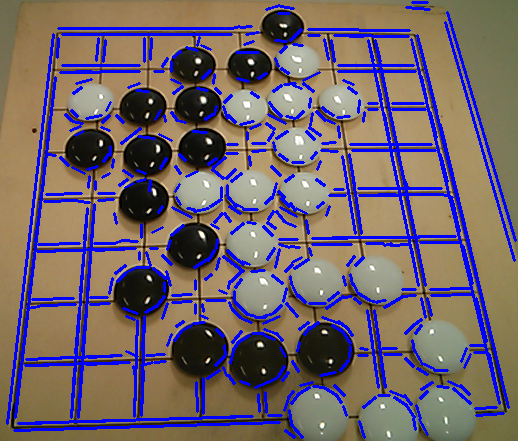
\includegraphics[width=\textwidth]{images/lsd_first.png}
			\label{fig:lsdPostprocessingFirst}
			\caption{Unfiltered LSD output}
		\end{subfigure}
		\hfill
		\begin{subfigure}{0.23\textwidth}
			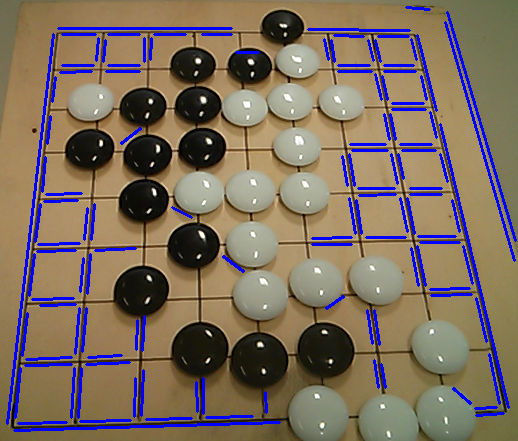
\includegraphics[width=\textwidth]{images/lsd_length.png}
			\label{fig:lsdPostprocessingLength}
			\caption{... filtered for line length,}
		\end{subfigure}
		\hfill
		\begin{subfigure}{0.23\textwidth}
			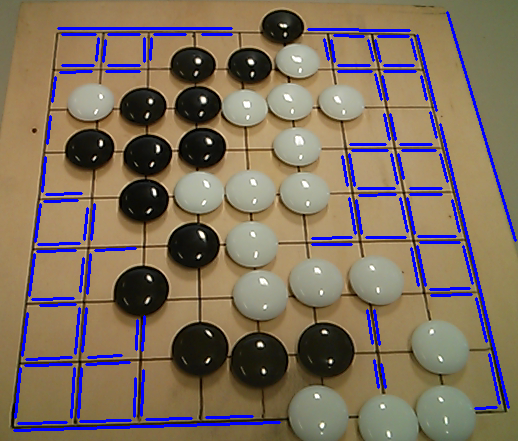
\includegraphics[width=\textwidth]{images/lsd_parallel.png}
			\label{fig:lsdPostprocessingParallel}
			\caption{... filtered for parallels, }
		\end{subfigure}
		\hfill
		\begin{subfigure}{0.23\textwidth}
			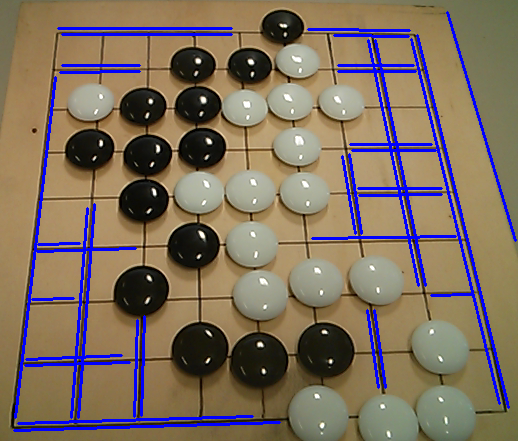
\includegraphics[width=\textwidth]{images/lsd_final.png}
			\label{fig:lsdPostprocessingFinal}
			\caption{and stitched and filtered for length}
		\end{subfigure}

		\caption{The postprocessing steps necessary for the LSD}
	\end{figure}


	\subsection{Using corner detectors}
	\label{detector-visible-corners}
	Another option to detect the intersection directly without line detection might be to use a corner detector. We tested the FAST \cite{rosten2006machine} detector on a slightly blurred image for this task. However it provides too many false positives to be of any use. Especially around black stones it is extremely unreliable. The ORB detector which uses FAST internally does not increase quality either.

	\section{Detecting occluded intersections}
	We know try to fill up intersections that could previously not be detected by finding the location of pieces additionally. Both methods that we tested need some preprocessing, though.

	To remove the lines and have only the pieces themselves remaining we tried thresholding the image. This works quite well for the black pieces. The white pieces on the other hand cannot be reliably detected this way. This is because the contrast between white pieces and the board is too low. We therefore turned to color images. We convert those from OpenCV's native BGR into HSV color space and threshold the value channel for black pieces, again with good results.

	%TODO: die zwei klammern neu formulieren, das ist ja grausam. am besten ganzen absatz.
	White pieces cannot be detected in the value channel because the contrast there is too low. In the other channels they remain hard to detect, too, as the white balance of the camera input is constantly being adjusted by the operating system. This leads to color aberrations when a player puts down a stone and his or her hand takes up lots of the image: the image will change its color temperature and white pieces become slightly blue. Often the aberration will be corrected after the hand leaves the image, but depending on the background this does not happen every time. Luckily the white pieces are well detectable under normal circumstances in the saturation channel (saturation of the pieces is low and of the board is high, hue is undefined) and when the color is shifted in the hue channel (saturation of the pieces and the board is low, hue of the pieces is low). We tried using fixed white balance settings by forcing camera parameters, but we could find none which worked under all tested illuminations.

	Therefore we threshold the saturation and the hue channel separately, count the non-zero responses and use the individual results only if at most 20\% of the image is below the threshold.

	This yields pretty good results, however there is still a lot of noise in the thresholded image. To reduce this we apply a Gaussian blur to the source image before thresholding and remove speckles afterwards by eroding and dilating the image slightly.

	Even still black pieces are being detected better, as we describe in TODO===TODO. However it is not very important for us to have a perfect detection ratio in this step, because the results are not used to generate the end result but only to fill in gaps in the intersections previously detected.
	\subsection{Using Hough circles}
	\label{detector-occluded-hough}
	Go pieces are relatively round and can be detected using Hough circles to some extent as long as the image is taken from a relatively high angle. If the camera is positioned near to the plane in which the board lies the circles become ellipses. In order to still match the pieces the threshold in the accumulator space beyond which a circle center will be detected has to be chosen quite low. This results in many false positives where noise is located by chance in some near-circle configuration.

	The centers of the detected circles are then added to intersections and duplicates (determined by their distance) are removed.

	\subsection{Using contours}
	\label{detector-occluded-contours}
	%TODO updaten
	Finding pieces with hough transformation is slow, though, and we were not contempt with the result to speed ratio. That is why we investigated further and chose to try analyzing the image topologically using OpenCV's \emph{findContours} function.

	We preprocess the image the same way as before. This results in blobs for each piece whose contours can be detected nicely. Those can then be fitted well into quadratic rectangles. If we encounter a rectangle which is about twice as long in one dimension as in the other, we split it in two. We then discard all contours whose bounding box is not more or less quadratic and filter the rectangles by their size.

	The centers of the detected squares are then added to intersections just like the centers of the circles when using hough transformation.

	\section{Calculating missing intersections}
	\label{detector-calculate}
	Having collected a set of probable intersections we now must fill in gaps where neither lines nor pieces have been detected. Also we need to somehow figure out which detected intersections are valid and actually are part of the board and which are simply intersections of grid lines with the outer edge of the board or other noise.

	First we calculate the average angle of the horizontal lines from the previous step and rotate the image to justify them. Then we select a number of intersections in the center of the board by selecting all intersections inside a square around the center. To do so, we assume the center of the board is the closest (detected or yet undetected) intersection to the center of the image. While this assumption can hardly be made in setups where the image is taken by bystanders or from randomly located cameras, we argue that when trying to record a game a user will be able to adjust the camera location accordingly. Another possibility could be to prompt the user for the center of the board, which is easily done via the touchscreen of the smart phone. We did not implement this approach for time reasons, but it should yield equal quality.

	%TODO: anzahl evaluieren und hier eintragen
	If the number of selected intersections is too small, we increase the window size and try again.

	Those intersections are now modeled as a subset of actual board intersections. We determine the median distance between neighboring intersections -- using the mean yielded worse results. Then we iterate row-wise over the selected intersections from the top left to the bottom right (to facilitate this we sort the intersections before selection). For every intersection we save the current row and column (on the board, not the image) and add a key point to our model at this location. If we encounter a gap between two intersection that is larger than the median distance we increase the column count accordingly. The same happens in y-direction with the row count. If we find an intersection is an outlier to the left we increase the column count of all previous key points accordingly.

	The interim result of this iteration is a submodel of the board with equidistant key points where every key point correspondents to a selected intersection.

	During the iteration we also add virtual intersections to fill in gaps in our intersection set. From this filled up intersection set we select the intersection closest to the image center and assume it is the intersection in the center of the board. Using the center intersection row and column count we can shift our model to the correct position within the board.

	Our updated interim result is now a submodel of the board located correctly inside the whole model, which we can feed into the RANSAC algorithm, as we made sure every key point corresponds to an intersection thus creating homography between the actual image and the hypothetical image of our modeled board. This serves three purposes. First, the RANSAC algorithm tolerates outliers, i.e. intersections which have been detected slightly wrong. Second, we can use the homography information to rectify subsequent images and increase detection quality. Lastly the transformation matrix can also be used to warp a complete model of the board and lay it onto the image. Now we know the location of every intersection -- including those, which have not been detected previously.

	\section{Postprocessing}
	\label{detector-postprocessing}

	\section{Classifying intersections}
	\label{detector-classifying}
	We can now evaluate the board at the intersections to find whether there's a piece there or not and if so of which color it is. The first step here is to use an adaptive threshold and to segment the board using a connect component analysis similarly to the preprocessing step. The result is a binary image showing only the lines and black pieces. Highlights within the black pieces from reflections are still a problem but can be removed well enough by erosion and dilution.

	For every intersection we calculate the average pixel value in a window and compare it to two thresholds, such that \begin{equation}
		\frac{\sum^{I,J}_{i=0,j=0}w(i,j)}{I*J} =
		\begin{cases}
		> T_{w} + C & \Rightarrow  \text{white}\\
		< T_{b} & \Rightarrow \text{black}\\
		\text{otherwise} & \Rightarrow \text{empty}
		\end{cases}
	\end{equation}
	where $C$ is a constant value that is added to the white threshold on the edge of the grid. This is necessary because the lines are not continued there and less black pixels from them are contributed.

	%TODO: evtl postprocessing (gleitender durchschnitt der intersections)
	%TODO: rotation der intersections
	%TODO: unsegmentation der intersections

\cleardoublepage
%!TEX root = ../Thesis.tex

\chapter{Creating the Android app}
\label{android}
	So far we have only described our detection algorithm, but not how to gather the data or how to interact with the user. Our goal was to create a simple user experience showcasing the algorithm rather than building a full featured app. Still we wanted to hide the technical details as far as useful to stay reasonably close to a usable end product.

	The app was deployed and developed for a \textit{Nexus 4} (also known as \textit{LG-E960}) running \textit{Android Lollipop 5.0.1} build LRX22C.

	\section{Tethering in the framework}
	\label{android-framework}
	\subsection{Adding the source dependencies}
	\label{android-framework-dependencies}
	OpenCV for Android is available since September 2011 so we will not describe in detail how we set it up. In short the process is as following. The Android bindings for OpenCV can be downloaded from the official site and be compiled into a library which can then be included into one's project's \textit{lib}-folder. Alternatively the framework can be set as a dependency in Eclipse Android Development Tool and let it handle the compilation and dependency resolution, which is how we included the library.

	One could build all the OpenCV native code for the framework oneself. This implies building it for every possible target architecture (ARMv6, ARMv7, x86...) and shipping it with the app. This creates large binaries, at the benefit of having a standalone application. The recommended way on the other hand is to depend on the \textit{OpenCV Manager} app and ask the user on first start to install it, if necessary. This manager will then download the correct OpenCV native binaries in the required version and share it between all applications needing it. We chose to do the latter, at least for our prototype.

	\subsection{Gathering data}
	\label{android-framework-gathering}
	On Android apps are structured into \textit{Activities}. Those roughly correspond to the screens visible to a user: If an app that has an overview screen, an editor screen and a preview screen, it will likely have three activities.

	Each activity is built out of \textit{Views} describing and implementing the user interface and this is where the OpenCV framework comes in: It offers a special \texttt{JavaCameraView}, which offers a callback to \texttt{CvCameraListener2} interfaces for delivery of CameraFrames and displays the frames on the screen. However it does not expose access to the camera and locks the device for itself. To have more control over the camera (for example we experimented with locking the exposure and white balance to fix the issue of color aberration under certain circumstances as described in \autoref{detector-occluded-hough}) we subclassed it into \texttt{CameraManipulatingView}. Our final setup comprises a \texttt{DetectorActivity} which implements the \texttt{CvCameraListener2} interface and uses a \texttt{CameraManipulatingView}.

	After startup we call the \textit{OpenCV Manager} to load an instance of OpenCV 2.4.3. Once that's done our native code library is loaded and we start receiving camera information from the \texttt{CameraManipulatingView} while still having access to camera parameters via it. We can retrieve images out of the camera information -- either in grayscale or RGBA color space.

	Each image is then compared to the last one. They are subtracted and if they differ significantly in more than 20 pixels, the resulting image is directly returned, thereby skipping the detector and improving FPS and energy consumption while the user moves the camera. It also pre-filters some frames in which too much movement occurs, for example because one player is putting down a piece.

	The user can choose between two activities on the top of the screen: Recording (detection) mode and replay mode. When the user is in detection mode and presses the record button the current illumination and white balance is fixed via the \texttt{CameraManipulatingView}. This improves the contrast between the board and the white pieces. As more and more white pieces are put on the board, the white balance would else shift and the contrast deteriorate.

	\section{Using the detector}
	\label{android-detector}
	When an image passes the movement filter it is being analyzed, for which there are two possible approaches. Either using Android OpenCV or the Java Native Interface (JNI) to call compiled C++ code. As the first is mainly a Java wrapper around C++ code, using it also involves costly JNI calls. Therefore it is more performant to implement the detector in C/C++ and have just one call into the detector. This is also how we chose to structure our application -- it is an easy way to increase performance. It means, however, that our application has to be compiled and shipped for every target architecture separately using the Android NDK.

	To really benefit from the performance increase we decided to use our detector as a black box and have only one call into it. The method is called \texttt{detect} and takes multiple parameters.

	While we could allocate memory in the native part of our application and release it when the app is stopped, it is much easier to request the memory in the Java part and let the garbage collector clean up the unneeded memory. Even for OpenCV matrices which have to be manually released this holds true, as another JNI call would be necessary in the \texttt{onStop} callback of the Activity. Therefore all input/output-parameters are allocated or at least declared in the Java class and filled or instantiated in the native part.

	The first and most obvious parameter to pass is the image to analyze. It is important to note that while OpenCV usually assumes that color images are in BGR(A)-format the Android bindings retrieve an RGBA-image from the camera. Thus, the image's color space has to be converted before passing it into the detector. As we encountered problems in numerous places when dealing with images whose color channels use 8-bit integers to encode their value, we decided to play it safe and switch to floating point channels at this stage, too. There might be concerns that due to differences in floating point precision some calculations might yield different results. We briefly looked into this and found that we either did no operation that needed this level of accuracy or it did not return different results.

	The detection result is being written into a \texttt{char} array with an entry for every intersection of the board. It contains a \texttt{0}, \texttt{b} or \texttt{w} character after detection, corresponding to an empty intersection, one with a black or with a white piece on it, respectively.

	In order to perform the postprocessing steps as noted in \autoref{detector-postprocessing} we need to pass the previously detected intersection back into the detector, which is done via a \texttt{MatOfPoint2f}. This is a special kind of OpenCV matrix, consisting of only one column and $n$ rows. It is used to quickly pass data between Java and native code. While Java lists would have to be copied matrices use the same memory in both environments, which allows seamless data exchange.

	All the other parameters are there to output information from the detector. Among them are lists of detected intersections, pieces and intersections -- all of which are there rather for debugging purposes than to give useful information to the user.

	As said before we set the exposure and white balance lock when starting to record. Still the computed intersections in two consecutive frames slightly differ. On the one hand this is a good thing: It helps dealing with specular highlights. On the other hand sometimes the detection result will deteriorate completely. Even though the detector does some sanity checks, displaying and saving the detection results directly would result in pieces ''flickering'' between being detected and not. To counteract this we count the number of times an intersection was classified as white or black in the last ten frames. If this counter reaches 5 or higher we assume a correct result and display it to the user. If the game is being recorded we also save two consecutive, aggregated and differing piece configurations in a list.

	\section{User interaction}
	\label{android-ui}
	\begin{figure}[h]
		\center
		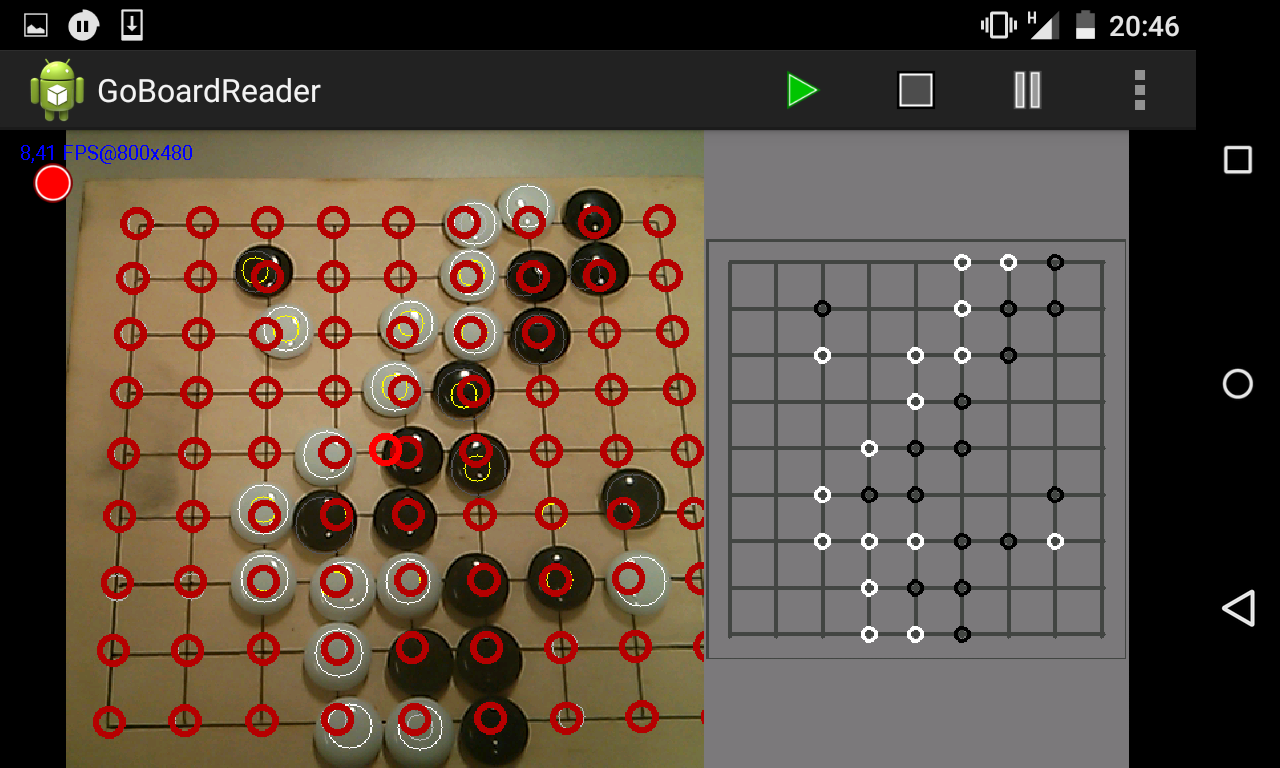
\includegraphics[width=0.7\textwidth]{images/android_ui.png}
		\caption{The app showing some debugging information and the detection result in a split screen while recording a game}
		\label{fig:android_ui}
	\end{figure}
	This information has to be displayed to the user. While often computer vision applications draw directly onto the analyzed image we decided to show the detected information separately and debugging output on the image, because we want to showcase a possible way how the app might be responding to the user and give him an insight of whether and how it's working.


	Android offers methods to draw custom views via \texttt{Canvas} and \texttt{Paint} objects similarly to OpenCV. In order to have a comparable experience when using the detector on a desktop computer and via the app we decided, however, to draw the result by cropping the input image and draw the result next to it using OpenCV when in detection mode.


\cleardoublepage
%!TEX root = ../Thesis.tex

\chapter{Evaluation}
	\section{Dataset}
	%Protocol
	\section{Kreuzungspunkte}
		\subsection{HOUGH}
		\subsection{LSD}
		\subsection{FAST}
	\section{Vorverarbeitung}
		\subsection{Gauss}
		\subsection{Informationen aus vorherigem Run}
\chapter{Ausblick}
\chapter{Zusammenfassung}

\cleardoublepage
%\include{chapters/chapter2}   % (\chapter{})
%\cleardoublepage
%\include{chapters/chapter7-ausblick}   % Ausblick (\chapter{Ausblick} TEXT)
%\cleardoublepage
%\include{chapters/chapter8-zusammenfassung}   % Zusammenfassung (\chapter{Zusammenfassung}  TEXT)
%\cleardoublepage

\appendix
\cleardoublepage
%\include{chapters/glossar}   % Glossar (\chapter{Glossar}  TEXT)
%\cleardoublepage

%%%%%%%%%%%%%%%%%%%%%%%%%%%%%%%%%%%%%%%%%%%%%%%%%%%%%%%%%%%%%%%%%%%%%%%%%%
% Diese Datei nicht veraendern!
%%%%%%%%%%%%%%%%%%%%%%%%%%%%%%%%%%%%%%%%%%%%%%%%%%%%%%%%%%%%%%%%%%%%%%%%%%
\addcontentsline{toc}{chapter}{\listfigurename}
\listoffigures
 % Bilderverzeichnis
\cleardoublepage
%%%%%%%%%%%%%%%%%%%%%%%%%%%%%%%%%%%%%%%%%%%%%%%%%%%%%%%%%%%%%%%%%%%%%%%%%%
% Diese Datei nicht veraendern!
%%%%%%%%%%%%%%%%%%%%%%%%%%%%%%%%%%%%%%%%%%%%%%%%%%%%%%%%%%%%%%%%%%%%%%%%%%
\addcontentsline{toc}{chapter}{\listtablename}
\listoftables
 % Tabellenverzeichnis
\cleardoublepage
%%%%%%%%%%%%%%%%%%%%%%%%%%%%%%%%%%%%%%%%%%%%%%%%%%%%%%%%%%%%%%%%%%%%%%%%%%
% Diese Datei nicht veraendern!
%%%%%%%%%%%%%%%%%%%%%%%%%%%%%%%%%%%%%%%%%%%%%%%%%%%%%%%%%%%%%%%%%%%%%%%%%%
\addcontentsline{toc}{chapter}{\bibname}
\bibliography{Thesis}
 % Literaturverzeichnis

\end{document}
